\section{Пространство $ \RN $.}

\subsection{Линейное евклидово пространство $ \RN $.}

Векторное пространство $G$ называется линейным над полем скаляров $H$, если определены алгебраические операции сложения и вычитания векторов в $G$, а также умножение векторов из $G$ на скаляры из $H$, удовлетворяющие соответствующим аксиомам, причём для $\forall x, y \in G$ и $\forall \lambda, \mu \in H \Rightarrow \left(\lambda x + \mu y \right) \in G$.

В дальнейшем будем рассматривать $n$-мерное векторное пространство $ \RN = \underbrace{ \mathbb{R} \times \mathbb{R} \times \ldots \times \mathbb{R}}_{\text{n раз}}$ (декартово произведение множеств), состоящее из всевозможных упорядоченных наборов из $n$ действительных чисел, т.е.
%\begin{equation*}
$ 	\RN = \{x = (x_1; x_2; \ldots; x_n) | \forall x_k \in \mathbb{R}, k = \overline{1, n} \}, $
%\end{equation*}
с операциями покомпонентного сложения и вычитания элементов (векторов).

Для $\forall x = \left(x_1; \ldots; x_n \right) \in \RN, \forall y = \left(y_1; \ldots; y_n \right) \in \RN$ полагая $ \lambda x + \mu y = (\lambda x_1 + \mu y_1, \lambda x_2 +$ 
$+ \mu y_2, \ldots, \lambda x_n + \mu y_n) \in \RN$, получим линейное пространство $\RN$ над полем действительных чисел $\mathbb{R}$.

Это линейное пространство $\RN$ называется евклидовым, если каждой паре $x, y \in \RN$ сопоставляется действительное число (скалярное произведение), обозначаемое $<x, y>$ и удовлетворяющее следующим аксиомам:
\begin{enumerate}
	\item Неотрицательность и невырожденность скалярного произведения: \\
	для $\forall x \in \RN \Rightarrow <x, x> \geqslant 0$, причём $<x, x> = 0 \Leftrightarrow x = \overline{0} = (0; 0; \ldots; 0) \in \RN$.
	\item Симметричность: \\
	для $\forall x, y \in \RN \Rightarrow <x, y> = <y, x>$.
	\item Линейность: \\
	для $\forall x, y, z \in \RN$ и $\forall \lambda, \mu \in \mathbb{R} \Rightarrow 
	< \lambda x + \mu y, z > = \lambda \cdot <x, z> + \mu <y, z>$.
\end{enumerate}
Из последней аксиомы при $\lambda = \mu = 0$ для $\forall z \in \RN$ в частности следует
\begin{equation*}
	<\overline{0}, z> = <0 \cdot x + 0 \cdot y, z> = 0 \cdot <x, z> + 0 \cdot <y, z> = 0.
\end{equation*}

\begin{theorem}[неравенство Коши — Буняковского]
	В линейном евклидовом пространстве $\RN$ для $\forall x, y \in \RN$ выполняется неравенство Коши — Буняковского
	\begin{equation}
	\label{lect01:koshibunIneq}
	\boxed{
		\left(<x, y>\right)^2 \leqslant (<x, x>) \cdot (<y, y>)}
	\end{equation}
\end{theorem}
\begin{proof}
	Для произвольных фиксированных $x, y \in \RN$ рассмотрим функцию \\
	$f(t) = (<tx + y, tx + y>) \geqslant 0$ действительной переменной $t \in \mathbb{R}$. В силу аксиом скалярного произведения, имеем 
	\begin{equation*}
	\begin{split}
	& f(t) = < tx, tx > + <tx, y> + <y, tx> + <y, y> = \\
	&= t^2 <x, x> + t<x, y> + t<y, x> + <y, y> = a t^2  + 2bt + c,
	\end{split}
	\end{equation*}
	где $a = \left(<x,x>\right) \geqslant 0, b = <x,y>, c = <y,y>$.
	
	Если $a = 0$, то $x = \overline{0}$, и, значит, $\left(<x,y>\right)^2 =  0 = 0 \cdot <y, y> = <x, x> \cdot <y,y>$, т.е. в этом случае неравенство  \eqref{lect01:koshibunIneq} выполняется.
	
	Пусть $a = (<x, x>) > 0$, т.е. $x \ne \overline{0}$. Тогда ветви параболы $f(t) = a t^2 + 2bt + c$ направлены вверх и сама она расположена полностью в верхней полуплоскости относительно оси абсцисс переменной $t \in \mathbb{R}$, т.к. для $\forall t \in \mathbb{R} \Rightarrow f(t) \geqslant 0$. Поэтому $D_1 = b^2 - ac \leqslant 0$, т.е. $b^2 \leqslant ac$, что равносильно \eqref{lect01:koshibunIneq}.\\
\end{proof}
\begin{consequence} (неравенство Минковского) \\
В линейном евклидовом пространстве $\RN$ для $\forall x, y \in \RN$ справедливо неравенство Минковского
	\begin{equation}
	\label{lect01:minkovskyIneq}
	\boxed{
		\sqrt{<x+y, x+y>} < \sqrt{<x, x>} + \sqrt{<y,y>}.
		}
	\end{equation}
\begin{proof}
	Используя \eqref{lect01:koshibunIneq} для $\forall x, y \in \RN$ получаем 
	\begin{equation*}
	\begin{split}
	& \sqrt{<x+y, x+y>} = \sqrt{<x,x> + 2 <x,y> + <y,y>} \leqslant \left[ \dfrac{ }{ }(<x,y>) \leqslant |<x,y>| \right] \leqslant \\
	& \leqslant \sqrt{<x,x> + 2 \abs{<x,y>} + <y,y>} \stackrel{\eqref{lect01:koshibunIneq}}\leqslant \left[
	|<x,y>| \leqslant \sqrt{<x,x> \cdot <y,y>} \dfrac{ }{ }\right] \leqslant \\
	& \leqslant \sqrt{\left(\sqrt{<x,x>}\right)^2 + 2 \sqrt{ <x,x> } \cdot \sqrt{ <y,y> } + \left(\sqrt{<y,y>}\right)^2} = \sqrt{\left(\sqrt{<x,x>} + \sqrt{<y,y>}\right)^2} = \\
	& = \sqrt{<x,x>} + \sqrt{<y,y>}.
	\end{split}	
	\end{equation*}
\end{proof}
\end{consequence}
\begin{note}
	В дальнейшем, как правило, в линейном пространстве $\RN$ будем использовать евклидово скалярное произведение, которое для простоты обозначим $x \cdot y = <x,y>$, и для которого для $\forall x = \left(x_1; x_2; \ldots; x_n\right) \in \RN, \forall y = \left(y_1; y_2; \ldots; y_n\right) \in \RN$ имеем
	\begin{equation}
	\label{lect01:innerproduct}
	\boxed{
		x \cdot y = x_1 y_1 + x_2 y_2 + \ldots + x_n y_n = \sum_{k=1}^{n}x_k y_k.}
	\end{equation}
	Нетрудно проверить, что \eqref{lect01:innerproduct} удовлетворяет всем аксиомам скалярного произведения (неотрицательность и невырожденность, симметричность, линейность). В этом случае для полученного евклидового линейного пространства $\RN$ с евклидовым скалярным произведением \eqref{lect01:innerproduct} неравенство Коши — Буняковского принимает вид
	\begin{equation}
	\label{lect01:koshibunIneq2}
	\boxed{
		\left(x_1 y_1 + \ldots + x_n y_n\right)^2 \leqslant \left(x_1^2 + \ldots + x_n^2\right)\left(y_1^2 + \ldots + y_n^2\right),}
	\end{equation}
	а неравенство Минковского даёт
	\begin{equation}
	\label{lect01:minkovskyIneq2}
	\boxed{
		\sqrt{\sum_{k=1}^{n} \left(x_k + y_k\right)^2} \leqslant \sqrt{\sum_{k=1}^{n} x_k^2} + \sqrt{\sum_{k=1}^{n} y_k^2},}
	\end{equation}
	где $\forall x_k, y_k \in \mathbb{R}, k = \overline{1, n}$.
\end{note}

\begin{exercise}
Выяснить, при каких условиях неравенства \eqref{lect01:koshibunIneq2} и \eqref{lect01:minkovskyIneq2} переходят в соответствующие равенства.	
\end{exercise}

\subsection{Нормированные и метрические пространства $ \RN $.}

Линейное пространство $ \RN $ будем называть нормированным, если имеется отображение
\begin{equation}
	\label{lect01:normaDisplay}
	\norma{\; . \;} \; \colon \; \RN \xrightarrow{} \mathbb{R},
\end{equation}
ставящее в соответствие для $ \forall x \in \RN $ действительное число $ \norma{x} \in \mathbb{R} $, и для которого выполнены следующие аксиомы нормы:
\begin{enumerate}
    \item {Невырожденность нормы}\\    
    $ \norma{x} = 0 \Leftrightarrow x = \overline{0} \in \RN $.
    \item {Однородность нормы}\\
    для $ \forall \; x \in \RN $ и $ \forall \lambda \in \mathbb{R} \Rightarrow \norma{\lambda x} = \abs{\lambda} \cdot \norma{x}$.
    \item {Неравенство треугольника для нормы}\\
    для $ \forall \; x, y \in \RN \Rightarrow \norma{x+y} \leqslant \norma{x} + \norma{y} $.
\end{enumerate}

Из этих аксиом при $ y = - x $ получаем
$ 0 = \norma{\overline{0}} = \norma{x + (-x)} \leqslant \norma{x} + \norma{-x} = \norma{x} + $ 
$ + \abs{-1} \cdot \norma{x} = \norma{x} + \norma{x} = 2 \norma{x}$, 
т. е. $ 2 \norma{x} \geqslant 0 $, и, значит, для $ \forall x \in \RN \Rightarrow \norma{x} \geqslant 0$. Поэтому любая норма \eqref{lect01:normaDisplay} в $ \RN $ также обладает свойством неотрицательности.

\begin{theorem}[о нормировании линейного евклидового пространства]
    Любое линейное евклидово пространство $ \RN $ нормируется с помощью естественной нормы
    \begin{equation}
        \label{lect01:naturalNorma}
        \begin{cases}	
        	\norma{x} = \sqrt{ < x, x > }, \\
            \forall \; x \in \RN.
        \end{cases}
    \end{equation}    
\end{theorem}

\begin{proof}
    На основании аксиом скалярного произведения в $ \RN $ проверим справедливость всех аксиом нормы для \eqref{lect01:naturalNorma}.
    
    Так как для $ \forall \; x \in \RN \Rightarrow (<x,x>) \geqslant 0 $, то, во-первых, отображение \eqref{lect01:naturalNorma} корректно определено, и, во-вторых,
    если $ \norma{x} = 0 $, то $ <x, x> \overset{\eqref{lect01:naturalNorma}}{=} 0$, т.е. $ x = \overline{0} $.
    Далее для $ \forall x \in \RN $ и $ \forall \lambda \in \mathbb{R} $ в силу линейности скалярного произведения из \eqref{lect01:naturalNorma} следует:    
    \begin{equation*}
        \norma{\lambda x} = \sqrt{< \lambda x, \lambda x >} = \sqrt{\lambda^2 < x, x >} = \abs{\lambda} \sqrt{<x,x>} = \abs{\lambda} \cdot \norma{x}.
    \end{equation*}
    
    Кроме того, используя неравенство Минковского \eqref{lect01:minkovskyIneq} для $ \forall \; x, y \in \RN $ получаем:
    \begin{equation*}
        \norma{x+y} \overset{\eqref{lect01:naturalNorma}}{=} \sqrt{<x+y, x+y>} \leqslant \sqrt{<x,x>} + \sqrt{<y,y>} = \norma{x} + \norma{y}.
    \end{equation*}    
\end{proof}

\begin{note}
    В случае линейного евклидового пространства $ \RN $ с евклидовым скалярным произведением \eqref{lect01:innerproduct} естественной нормой будет:
    \begin{equation*}
        \begin{cases}
        	\norma{x} = \sqrt{x_1^2 + x_2^2 + \ldots + x_n^2}, \\        	
            \forall \; x = (x_1, x_2, \ldots, x_n) \in \RN.
        \end{cases}
    \end{equation*}
\end{note}

В этом случае для простоты вместо $ \norma{x} $ будем писать $ \abs{x} = \left(\dsum_{k=1}^{n} x_k^2\right)^{\frac{1}{2}} $.

\begin{exercise}
    Показать, что для $ \forall \;x, y \in \RN $ следует:
    \begin{equation*}
    	\abs{\abs{x} - \abs{y}} \leqslant \abs{x \pm y} \leqslant \abs{x} + \abs{y}
    \end{equation*}
\end{exercise}

Линейное пространство $ \RN $ будем называть \important{метрическим}, если имеется отображение:
\begin{equation}
    \label{lect01:metricDisplay}
	\rho \colon \RN \times \RN \rightarrow \mathbb{R},
\end{equation}
ставящее в соответствие для $ \forall \; x, y \in \RN $ действительное число $ \rho(x,y) \in \mathbb{R} $, удовлетворяющее следующим аксиомам расстояния:
\begin{enumerate}
    \item {Неотрицательность расстояния}:\\
    для $\forall \; x, y \in \RN \Rightarrow \rho (x, y) \geqslant 0 $, причём $ \rho (x, y) = 0  \Leftrightarrow x = y $.
    \item {Симметричность расстояния}:\\
    для $\forall \; x, y \in \RN \Rightarrow \rho (x, y) =  \rho (y, x)$.
    \item {Неравенство треугольника для расстояния}:\\
    для $\forall \; x, y, z \in \RN \Rightarrow \rho (x, y) \leqslant \rho(x, z) + \rho (z, y)$.
\end{enumerate}

В дальнейшем линейное метрическое пространство $ \RN $ с используемой метрикой \eqref{lect01:metricDisplay} кратко будем обозначать $ (\RN, \rho) $.

\begin{theorem}[о метризируемости произвольного линейного нормированного пространства $ \RN $]
	Любое линейное нормированное пространство $ \RN $ метризируемо с помощью естественного расстояния
    \begin{equation}
        \label{lect01:naturalDistance}
        \begin{cases}
        	\rho (x, y) = \norma{x-y}, \\
            \forall \; x, y \in \RN.
        \end{cases}
    \end{equation}
\end{theorem}
\begin{proof}
    В силу аксиом нормы для $ \forall \; x, y \in \RN $, во-первых, имеем
    \begin{equation*}
    	\rho(x, y) \overset{\eqref{lect01:naturalDistance}}{=} \norma{x-y} \geqslant 0,
    \end{equation*}
    причём $ \rho(x,y)=0 \Leftrightarrow \norma{x-y} = 0 \Leftrightarrow x-y = \overline{0} \Leftrightarrow x = y $. Во-вторых, получаем 
    \begin{equation*}
    	\rho(x,y) \overset{\eqref{lect01:naturalNorma}}{=} \norma{-(y-x)} = \abs{-1} \cdot \norma{y-x} = \norma{y-x} = \rho(y, x)
    \end{equation*}
    И, в-третьих, из неравенства треугольника для нормы для $ \forall \; x,y,z \in \RN $ следует
    \begin{equation*}
    	\rho(x, y) \overset{\eqref{lect01:naturalNorma}}{=} \norma{(x-z) + (z-y)} \leqslant \norma{x-z} + \norma{z-y} = \rho(x,z) + \rho(z, y)
    \end{equation*}
\end{proof}

\newpage
\begin{notes}
    \item Для линейного евклидового пространства $ \RN $ с евклидовой нормой
    \begin{equation*}
	    \begin{cases}
			\abs{x} = \norma{x} = \left(\dsum_{k=1}^{n} x_k^2\right)^{\dfrac{1}{2}}, \\
            \forall \; x = (x_1, x_2, \ldots, x_n) \in \RN
        \end{cases}
    \end{equation*}
    на основании \eqref{lect01:naturalDistance} имеем евклидово расстояние 
    \begin{equation}
        \label{lect01:euclidianDistance}
        \begin{cases}
        	\rho(x,y) = \abs{x-y} = \left(\dsum_{k=1}^{n} (x_k-y_k)^2\right)^{\dfrac{1}{2}}, \\
            \forall \; x = (x_1, x_2, \ldots, x_n) \in \RN, \\
            \forall \; y = (y_1, y_2, \ldots, y_n) \in \RN.
        \end{cases}
    \end{equation}    
    В дальнейшем это расстояние \eqref{lect01:euclidianDistance} будем обозначать 
    \begin{equation*}
        d(x,y) = \rho(x,y) \overset{\eqref{lect01:euclidianDistance}}{=} \left(\dsum_{k=1}^{n} (x_k-y_k)^2\right)^{\dfrac{1}{2}},
    \end{equation*}
    а получаемое линейное евклидово метрическое пространство $ \RN $с этим евклидовым расстоянием также будем записывать в виде $ (\RN, d) $.
    \item Кроме метризируемости линейного нормированного пространства $ \RN $ с помощью естественной метрики \eqref{lect01:naturalDistance}, линейное пространство $ \RN $ метризируемо, например, с помощью тривиальной метрики 
    \begin{equation*}
        \rho_0(x,y) =
        \begin{cases}
            1, \text{ если } x \neq y,\\
            0, \text{ если } x = y.
        \end{cases}
    \end{equation*}
    
    Иногда наряду с пространством $ (\RN, d) $ удобнее использовать также метрические пространства $ (\RN, \rho_1) $ и $ (\RN, \rho_2) $ соответственно с октаэдрической метрикой
    \begin{equation*}
    	\rho_1(x, y) = \dsum_{k=1}^{n} \abs{x_k - y_k}
    \end{equation*}
    и кубической метрикой
    \begin{equation*}
      	\rho_2(x, y) = \max_{1 \leqslant k \leqslant n} \abs{x_k - y_k}
    \end{equation*}
    где $ \forall \; x = (x_1, x_2, \ldots, x_n) \in \RN $ и $ \forall \; y = (y_1, y_2, \ldots, y_n) \in \RN $.
\end{notes}

\begin{exercise}
    Доказать, что для тривиальной метрики, октаэдрической метрики и кубической метрики выполняются все аксиомы расстояния.
\end{exercise}

\subsection{Множества и окрестности в $ \RN $}

В дальнейшем в линейном метрическом пространстве $\left( \RN, \rho \right)$ для записи его элементов (векторов) будем использовать не только малые буквы
$\ldots, x, y, z, \ldots$, но и большие $\ldots, K, L, M, \ldots$, а сами элементы также будем называть точками.

Открытым шаром $B_r (x_0)$ радиуса $r > 0$ с центром в $x_0$ из $\left( \RN, \rho \right)$ будем называть \\множество
\begin{equation*}
	B_r (x_0) = \{x \in \RN | \rho (x, x_0) < r\},
\end{equation*}
а замкнутым шаром $\overline{B_r}(x_0)$ — множество
\begin{equation*}
\overline{B_r}(x_0) = \{x \in \RN | \rho (x, x_0) \leqslant r\}.
\end{equation*}
Очевидно, что
\begin{equation*}
\overline{B_r}(x_0) = B_r (x_0) \cup S_r (x_0),
\end{equation*}
где $S_r (x_0)$ является $n$-мерной сферой в $\left( \RN, \rho \right)$, т.е.
\begin{equation*}
S_r (x_0) = \{x \in \RN | \rho (x, x_0) = r\}.
\end{equation*}
Шары $B_r (x_0)$ и $\overline{B_r}(x_0)$ будем также соответственно называть открытыми и замкнутыми $r$-окрестностями для $x_0 \in \RN$, а в случае, когда размеры этих окрестностей несущественны и фиксированы, будем их обозначать для краткости как $V(x_0) = B_r (x_0)$ и $ \overline{V}(x_0) = \overline{B_r}(x_0)$.

\begin{statement}{Примеры}
	Рассмотрим пространство $\left(\RN, d \right)$.
	\begin{enumerate}
		\item Если $n = 1$, то для $\forall x_0 \in \mathbb{R}$ и $\forall x \in \mathbb{R} \Rightarrow d(x, x_0) = \abs{x - x_0}$.
		
		Поэтому в данном случае открытым шаром с центром в $x_0$ и радиуса $r > 0$ будет
		\begin{equation*}
			B_r (x_0) = \defineset{x \in \mathbb{R} \; \dfrac{ }{ }}{\dfrac{ }{ } \abs{x - x_0} < r} = ]x_0 - r; x_0 + r[
		\end{equation*}
		и замкнутым шаром является
		\begin{equation*}
		\overline{B_r} (x_0) = \defineset{x \in \mathbb{R} \; \dfrac{ }{ }}{\dfrac{ }{ } \abs{x - x_0} \leqslant r} = [x_0 - r; x_0 + r]
		\end{equation*}
		Одномерная сфера будет состоять из двух чисел $S_r(x_0) = \{x_0 - r; x_0 + r\}$.
		
		Геометрически получаем
		
		\begin{center}
			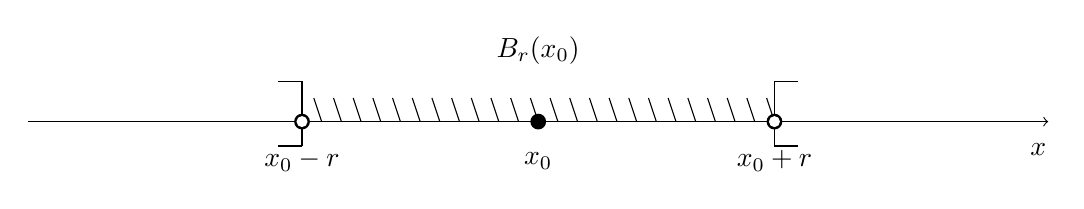
\begin{tikzpicture}
			\coordinate (left) at (-0.3 * \paperwidth, 0.0);
			\coordinate (right) at (0.3 * \paperwidth, 0.0);
			\coordinate (center) at (0, 0);
			\coordinate (delta) at(4.0, 0);
			\coordinate (delta2) at(3.0, 0);
			\coordinate (delta3) at(-3.0, 0);
			\coordinate (letterdeltabottom) at(0, -0.5);
			\coordinate (letterdeltatop) at(0.0, 0.5);
			
			\draw[->] (center -| left) -- (center -| right);
			\foreach \x in {-2.75, -2.5, ..., 3.0}
			\draw[xshift=\x cm] (0.0, 0.0) -- (-0.1, 0.3);
			\fill[black] (-3.0, 0) circle(0.1);
			\fill[white] (-3.0, 0) circle(0.07);
			%\fill[black] (center) ++ (delta) circle(0.12);
			\fill[black] (center) ++ (center) circle(0.1);
			\fill[black] (center) ++ (delta2) circle(0.1);
			\fill[white] (center) ++ (delta2) circle(0.07);
			\draw (0, 0.4) ++ (letterdeltatop) node {$ \boxed{B_r(x_0)} $};
			\draw (center) ++ (letterdeltabottom) node {$x_0$};
			\draw (center) ++ (delta2) ++ (letterdeltabottom) node {$x_0 + r$};
			\draw (center) ++ (delta3) ++ (letterdeltabottom) node {$x_0 - r$};
			\draw (3.35, 0.15) ++ (delta2) ++ (letterdeltabottom) node {$x$};
			\draw[fill=black] (-3.0, 0.07) -- (-3.0, 0.51);
			\draw[fill=black] (-3.0, 0.51) -- (-3.3, 0.51);
			\draw[fill=black] (-3.0, -0.07) -- (-3.0, -0.31);
			\draw[fill=black] (-3.0, -0.31) -- (-3.3, -0.31);
			\draw[fill=black] (3.0, 0.07) -- (3.0, 0.51);
			\draw[fill=black] (3.0, 0.51) -- (3.3, 0.51);
			\draw[fill=black] (3.0, -0.07) -- (3.0, -0.31);
			\draw[fill=black] (3.0, -0.31) -- (3.3, -0.31);
			\end{tikzpicture}
		\end{center}
		
		\begin{center}
			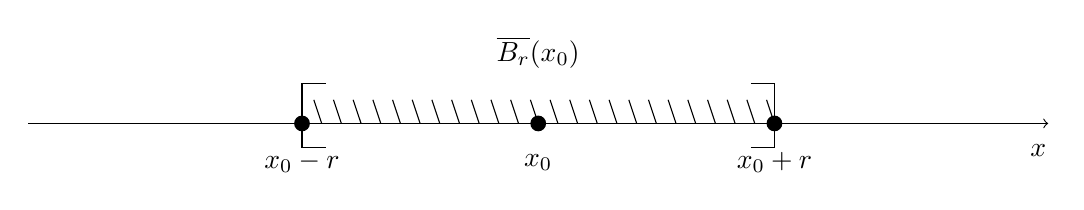
\begin{tikzpicture}
			\coordinate (left) at (-0.3 * \paperwidth, 0.0);
			\coordinate (right) at (0.3 * \paperwidth, 0.0);
			\coordinate (center) at (0, 0);
			\coordinate (delta) at(4.0, 0);
			\coordinate (delta2) at(3.0, 0);
			\coordinate (delta3) at(-3.0, 0);
			\coordinate (letterdeltabottom) at(0, -0.5);
			\coordinate (letterdeltatop) at(0.0, 0.5);
			
			\draw[->] (center -| left) -- (center -| right);
			\foreach \x in {-2.75, -2.5, ..., 3.0}
			\draw[xshift=\x cm] (0.0, 0.0) -- (-0.1, 0.3);
			\fill[black] (-3.0, 0) circle(0.1);
			%\fill[white] (-3.0, 0) circle(0.07);
			%\fill[black] (center) ++ (delta) circle(0.12);
			\fill[black] (center) ++ (center) circle(0.1);
			\fill[black] (center) ++ (delta2) circle(0.1);
			%\fill[white] (center) ++ (delta2) circle(0.07);
			\draw (0, 0.4) ++ (letterdeltatop) node {$\boxed{\overline{B_r}(x_0)}$};
			\draw (center) ++ (letterdeltabottom) node {$x_0$};
			\draw (center) ++ (delta2) ++ (letterdeltabottom) node {$x_0 + r$};
			\draw (center) ++ (delta3) ++ (letterdeltabottom) node {$x_0 - r$};
			\draw (3.35, 0.15) ++ (delta2) ++ (letterdeltabottom) node {$x$};
			\draw[fill=black] (-3.0, 0.07) -- (-3.0, 0.51);
			\draw[fill=black] (-3.0, 0.51) -- (-2.7, 0.51);
			\draw[fill=black] (-3.0, -0.07) -- (-3.0, -0.31);
			\draw[fill=black] (-3.0, -0.31) -- (-2.7, -0.31);
			\draw[fill=black] (3.0, 0.07) -- (3.0, 0.51);
			\draw[fill=black] (3.0, 0.51) -- (2.7, 0.51);
			\draw[fill=black] (3.0, -0.07) -- (3.0, -0.31);
			\draw[fill=black] (3.0, -0.31) -- (2.7, -0.31);
			\end{tikzpicture}
		\end{center}
		
		\begin{center}
			\begin{tikzpicture}
			\coordinate (left) at (-0.3 * \paperwidth, 0.0);
			\coordinate (right) at (0.3 * \paperwidth, 0.0);
			\coordinate (center) at (0, 0);
			\coordinate (delta) at(4.0, 0);
			\coordinate (delta2) at(3.0, 0);
			\coordinate (delta3) at(-3.0, 0);
			\coordinate (letterdeltabottom) at(0, -0.5);
			\coordinate (letterdeltatop) at(0.0, 0.5);
			
			\draw[->] (center -| left) -- (center -| right);
			%\foreach \x in {-2.75, -2.5, ..., 2.75}
			%\draw[xshift=\x cm] (0.0, 0.0) -- (-0.1, 0.3);
			%\fill[black] (-3.0, 0) circle(0.1);
			%\fill[white] (-3.0, 0) circle(0.07);
			%\fill[black] (center) ++ (delta) circle(0.12);
			%\fill[black] (center) ++ (center) circle(0.1);
			%\fill[black] (center) ++ (delta2) circle(0.1);
			%\fill[white] (center) ++ (delta2) circle(0.07);
			\draw (0, 0.4) ++ (letterdeltatop) node {$ \boxed{S_r(x_0)} $};
			%\draw (center) ++ (letterdeltabottom) node {$x_0$};
			\draw (center) ++ (delta2) ++ (letterdeltabottom) node {$x_0 + r$};
			\draw (center) ++ (delta3) ++ (letterdeltabottom) node {$x_0 - r$};
			\draw (3.35, 0.15) ++ (delta2) ++ (letterdeltabottom) node {$x$};
			\draw[fill=black] (-3.1, -0.1) -- (-2.9, 0.1);
            \draw[fill=black] (-3.0, -0.15) -- (-3.0, 0.15);
			\draw[fill=black] (-2.9, -0.1) -- (-3.1, 0.1);
			\draw[fill=black] (3.1, -0.1) -- (2.9, 0.1);
            \draw[fill=black] (3.0, -0.15) -- (3.0, 0.15);
			\draw[fill=black] (2.9, -0.1) -- (3.1, 0.1);
			\end{tikzpicture}
		\end{center}
		
		\item Пусть $n = 2$. Считая, что в $\mathbb{R}^2$ введена прямоугольная декартова система координат $Oxy$ имеем
		\begin{equation*}
			d(M, M_0) = \sqrt{(x-a)^2 + (y-b)^2}
		\end{equation*}
		где $M_0(a; b) \in \mathbb{R}^2$ и $M(x; y) \in \mathbb{R}^2$.
		
		В этом случае открытым шаром $B_r(M_0)$ будет соответствующий открытый круг
		\begin{equation*}
			B_r (M_0) = \{ (x, y) \in \mathbb{R}^2 | (x-a)^2 + (y-b)^2 < r^2 \},
		\end{equation*}
		а замкнутым шаром $\overline{B_r} (M_0)$ является замкнутый круг
		\begin{equation*}
		\overline{B_r} (M_0) = \{ (x, y) \in \mathbb{R}^2 | (x-a)^2 + (y-b)^2 \leqslant r^2 \}
		\end{equation*}
		Сфера
		\begin{equation*}
			S_r (M_0) = \{ (x, y) \in \mathbb{R}^2 | (x-a)^2 + (y-b)^2 = r^2 \}
		\end{equation*}
		представляет собой окружность с центром в $M_0(a; b)$ и радиуса $r > 0$.
		
		Геометрически получаем 
				\begin{center}
		\begin{tikzpicture}
			\coordinate (left) at (-1.0, 0.0);
			\coordinate (right) at (4.0, 0.0);
			\coordinate (top) at (0.0, 3);
			\coordinate (bottom) at (0.0, -1.0);
			\coordinate (center) at (0.0, 0.0);
			\draw[->] (left) -- (right);
			\draw[->] (bottom) -- (top);
			\draw (center) node[anchor=north east] {$O$};
			\draw (right) node[anchor=north] {$x$};
			\draw (top) node[anchor=west] {$y$};
			%\fill [black] (1.5, 1.5) circle (20pt);
			%\fill [white] (1.5, 1.5) circle (19pt);
			% Bottom part of plot
			%\draw[black, dashed] (1.5,1.5) circle (19pt);
			\draw [pattern = north west lines, pattern color=black, dashed] (1.5,1.5) circle (19pt);
			\draw[fill=black, dashed] (0, 2.2) -- (1.5, 2.2);
			\draw[fill=black, dashed] (0, 1.5) -- (1.5, 1.5);
			\draw[fill=black, dashed] (0, 0.8) -- (1.5, 0.8);
			\draw[fill=black, dashed] (1.5, 0) -- (1.5, 1.5);
			\draw[fill=black, dashed] (0.8, 1.5) -- (0.8, 0);
			\draw[fill=black, dashed] (2.2, 1.5) -- (2.2, 0);
			\draw (2.2,1.5) node[anchor=west] {$B_r(M_0)$};
			\fill [black] (1.5,1.5) circle (2pt);
			\fill [black] (1.5,0) circle (2pt);
			\fill [black] (0,0.8) circle (2pt);
			\fill [black] (0,2.2) circle (2pt);
			\fill [black] (0, 1.5) circle (2pt);
			\fill [black] (0.8,0) circle (2pt);
			\fill [black] (2.2, 0) circle (2pt);
			\draw (1.37,1.37) node[anchor=south west] {$\boldsymbol{M_0}$};
			\draw (0.8,0) node[anchor=north] {$a-r$};
			\draw (1.5,-0.06) node[anchor=north] {$a$};
			\draw (2.2,0) node[anchor=north] {$a+r$};
			\draw (0, 0.8) node[anchor=east] {$b-r$};
			\draw (-0.06, 1.5) node[anchor=east] {$b$};
			\draw (0, 2.2) node[anchor=east] {$b+r$};
			\end{tikzpicture}
		\end{center}
		
		\begin{center}
			\begin{tikzpicture}
			\coordinate (left) at (-1.0, 0.0);
			\coordinate (right) at (4.0, 0.0);
			\coordinate (top) at (0.0, 3);
			\coordinate (bottom) at (0.0, -1.0);
			\coordinate (center) at (0.0, 0.0);
			\draw[->] (left) -- (right);
			\draw[->] (bottom) -- (top);
			\draw (center) node[anchor=north east] {$O$};
			\draw (right) node[anchor=north] {$x$};
			\draw (top) node[anchor=west] {$y$};
			%\fill [black] (1.5, 1.5) circle (20pt);
			%\fill [white] (1.5, 1.5) circle (19pt);
			% Bottom part of plot
			%\draw[black, dashed] (1.5,1.5) circle (19pt);
			\draw [pattern = north west lines, pattern color=black] (1.5,1.5) circle (19pt);
			\draw[fill=black, dashed] (0, 1.5) -- (1.5, 1.5);
			\draw[fill=black, dashed] (1.5, 0) -- (1.5, 1.5);
			\draw (2.2,1.5) node[anchor=west] {$\overline{B_r}(M_0)$};
			\fill [black] (1.5,1.5) circle (2pt);
			\fill [black] (1.5,0) circle (2pt);
			\fill [black] (0, 1.5) circle (2pt);
			\draw (1.37,1.37) node[anchor=south west] {$\boldsymbol{M_0}$};
			\draw (1.5,-0.06) node[anchor=north] {$a$};
			\draw (-0.06, 1.5) node[anchor=east] {$b$};
			\end{tikzpicture}
		\end{center}
		\begin{center}
			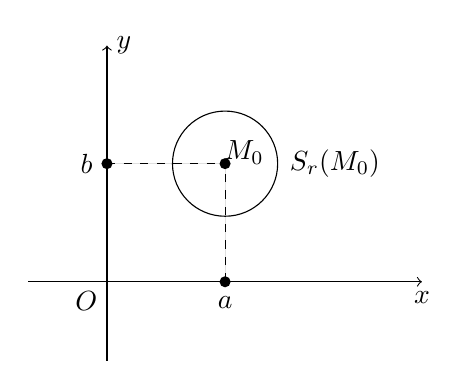
\begin{tikzpicture}
			\coordinate (left) at (-1.0, 0.0);
			\coordinate (right) at (4.0, 0.0);
			\coordinate (top) at (0.0, 3);
			\coordinate (bottom) at (0.0, -1.0);
			\coordinate (center) at (0.0, 0.0);
			\draw[->] (left) -- (right);
			\draw[->] (bottom) -- (top);
			\draw (center) node[anchor=north east] {$O$};
			\draw (right) node[anchor=north] {$x$};
			\draw (top) node[anchor=west] {$y$};
			%\fill [black] (1.5, 1.5) circle (20pt);
			%\fill [white] (1.5, 1.5) circle (19pt);
			% Bottom part of plot
			%\draw[black, dashed] (1.5,1.5) circle (19pt);
			\draw (1.5,1.5) circle (19pt);
			\draw[fill=black, dashed] (0, 1.5) -- (1.5, 1.5);
			\draw[fill=black, dashed] (1.5, 0) -- (1.5, 1.5);
			\draw (2.2,1.5) node[anchor=west] {$S_r(M_0)$};
			\fill [black] (1.5,1.5) circle (2pt);
			\fill [black] (1.5,0) circle (2pt);
			\fill [black] (0, 1.5) circle (2pt);
			\draw (1.37,1.37) node[anchor=south west] {$\boldsymbol{M_0}$};
			\draw (1.5,-0.06) node[anchor=north] {$a$};
			\draw (-0.06, 1.5) node[anchor=east] {$b$};
			\end{tikzpicture}
		\end{center}
		
		\item Аналогично для $n = 3$ в пространстве $(\mathbb{R}^3, d)$ для $M_0 (a, b, c) \in \mathbb{R}^3$ и $M(x, y, z) \in \mathbb{R}^3$ имеем
		\begin{equation*}
		d(M, M_0) = \sqrt{(x-a)^2 + (y-b)^2 + (z-c)^2}
		\end{equation*}
		и, значит,	

		\begin{enumerate}
			\item $B_r (M_0) = \{ (x, y, z) \in \mathbb{R}^2 | (x-a)^2 + (y-b)^2 + (z-c)^2 < r^2 \}$ — открытый шар в $\mathbb{R}^3$ с центром в $M_0$ и радиуса $r > 0$.
			\item $\overline{B_r} (M_0) = \{ (x, y, z) \in \mathbb{R}^3 | (x-a)^2 + (y-b)^2 + (z-c)^2 \leqslant r^2 \}$ — соответствующий замкнутый шар в $\mathbb{R}^3$.
			\item $S_r (M_0) = \{ (x, y, z) \in \mathbb{R}^3 | (x-a)^2 + (y-b)^2 + (z-c)^2 = r^2 \}$ — сфера в $\mathbb{R}^3$.
		\end{enumerate}
	\end{enumerate}
\end{statement}

\begin{exercise}
	Для $n = 1, 2, 3$ выяснить геометрический смысл множеств $B_r(M_0), \overline{B_r}(M_0)$ и $S_r (M_0)$ в пространствах $(\RN, \rho_1)$ и $(\RN, \rho_2)$ соответственно с октаэдрической и кубической метриками.
\end{exercise}

\begin{note}
	Кроме полных окрестностей $B_r(M_0)$ и $\overline{B_r}(M_0)$ в $(\RN, \rho)$ будем также использовать выколотые $r$-окрестности точки $M_0 \in \RN$, т.е. соответственно множества $\dot{B_r}(M_0) = $\\
	$ = B_r(M_0) \setminus \{M_0\}$ и $\dot{\overline{B_r}}(M_0) = \overline{B_r}(M_0) \setminus \{M_0\}$, которые для краткости иногда будем обозначать $\dot{V}(M_0) = \dot{B_r}(M_0)$ и $\dot{\overline{V}}(M_0) =\dot{\overline{B_r}}(M_0)$.
	
	Точку $M_0 \in D$ считаем изолированной для множества $D \subset \RN$, если $ \exists \; V (M_0) \subset \RN $, где нет других точек из $D$, кроме $M_0$.
	
	Точку $M_0 \in \RN$ будем называть предельной для множества $D \subset \RN$, если в $\forall \; V (M_0) \subset \RN$ есть точки из $D$, отличные от $M_0$. Очевидно, что любая изолированная точка множества $D \subset \RN$ не будет предельной для $D$.
	
	Точка $M_0 \in \RN$ называется внутренней точкой для $D \subset \RN$, если $\exists V (M_0) \subset D$.
	
	Точку $M_0 \in \RN$ будем называть граничной для множества $D \subset \RN$, если $\forall V (M_0) \subset \RN$ есть точки как принадлежащие $D$, так и не входящие в $D$.
	
	Множество всех граничных точек для $D \subset \RN$ называют границей множества $D$ и обозначают $\partial D$.
    
	Для $\forall D \subset \RN$ множество $\overline{D} = \partial D \cup D$ будем называть замыканием множества $D$. Множество $D \subset \RN$ считают замкнутым в $\RN$, если $\overline{D} = D$.
\end{note}

Можно показать, что множество $D \subset \RN$ будет замкнутым в $\RN$ тогда и только тогда, когда все его предельные точки входят в $D$.

Множество $D \subset \RN$ называют открытым в $\RN$, если для $\forall M_0 \in D \Rightarrow M_0$ —  внутренняя точка $D$. Нетрудно показать, что множество $D \subset \RN$ будет открытым в $\RN$ тогда и только тогда, когда его дополнение $\left( \RN \setminus D \right)$ замкнуто в $\RN$.
	

Открытые множества в $\RN$ обладают следующими основными свойствами:\\
1. Все $\RN$ и пустое множество $\emptyset$ являются открытыми в $\RN$;\\
2. Объединение \important{любого} числа открытых множеств в $\RN$ будет открытым множеством в $\RN$;\\
3. Пересечение \important{конечного} числа открытых множеств в $\RN$ является открытым множеством в $\RN$.
\newpage

\begin{note}
	Аналогичными свойствами обладают замкнутые множества в $\RN$:
\end{note}
\begin{enumerate}
	\item Всё $\RN$ и $\emptyset$ замкнуты в $\RN$;
	\item Объединение \important{любого} числа замкнутых множеств в $\RN$ является замкнутым множеством в $\RN$;
	\item Пересечение \important{конечного} числа замкнутых множеств в $\RN$ является замкнутым множеством в $\RN$.
\end{enumerate}

В дальнейшем множество $D \subset \RN$ будем называть ограниченным в линейном метрическом пространстве $\left( \RN, \rho \right)$, если все точки из $D$ расположены внутри некоторого $n$-мерного шара конечного радиуса.

\begin{exercise}
	Показать, что на множестве действительных чисел функция
	\begin{equation*}
	\rho (x, y) = \dfrac{\abs{x-y}}{1 + \abs{x-y}}, \forall x, y \in \mathbb{R},
	\end{equation*}
	удовлетворяет всем аксиомам расстояния и при этом в получаемом метрическом пространстве $\left(\mathbb{R}, \rho \right)$ все множества (даже бесконечные промежутки) будут ограниченными.
\end{exercise}

$  $\newline

%\begin{note}
	Любое ограниченное замкнутое множество $D \subset \RN$ метрического пространства $\left(\RN, \rho \right)$ называется компактом в $\RN$. Множество $D \subset \RN$ считается связным, если любые две точки $M_1, M_2 \in D$ можно соединить некоторой непрерывной \\
	линией $\ell = \arc{M_1 M_2} \; \subset D$, т.е. имеющей параметризацию 
	\begin{equation*}
	\ell = \left\{ \nullFrac x= x(t) \in \RN | x(t) = (x_1 (t); \ldots; x_n (t) ), t \in [\alpha; \beta] \nullFrac \right\},
	\end{equation*}
	где $\forall x_k (t)$ — непрерывные функции от $t \in [\alpha; \beta], k = \overline{1, n}$, для которых $x(\alpha) = M_1$ и ${x(\beta) = M_2.}$ 
    Открытое связное множество $D \in \RN$ в метрическом пространстве $\left(\RN, \rho \right)$ называют областью в $\RN$, а его замыкание $\overline{D}$ называют замкнутой областью в $\RN$.
%\end{note}

$ $\newpage$   $